\documentclass[tikz,border=8pt]{standalone}
% Shared look for every TikZ diagram. Load with \input{../../tools/tikz-style.tex}
\usepackage[T1]{fontenc}
\usepackage{lmodern}
\renewcommand{\sfdefault}{lmr}  % diagrams use the same serif as the text
\usetikzlibrary{arrows.meta, positioning, shapes.geometric, calc, fit, backgrounds}
\definecolor{cblue}{HTML}{4C78A8}
\definecolor{corange}{HTML}{F58518}
\definecolor{cgreen}{HTML}{54A24B}
\definecolor{cred}{HTML}{E45756}
\definecolor{cpurple}{HTML}{B279A2}
\definecolor{cgrey}{HTML}{6B6B6B}
\tikzset{
  every picture/.style={font=\sffamily, line width=1.2pt},
  box/.style={draw=#1, fill=#1!12, rounded corners=4pt, align=center, inner sep=7pt, minimum height=1.1cm},
  box/.default=cgrey,
  arrow/.style={-{Stealth[length=3mm]}, draw=cgrey, line width=1.4pt},
  title/.style={font=\sffamily\bfseries\Large},
  note/.style={font=\sffamily\small, text=cgrey, align=center},
}
\AtBeginDocument{\hyphenpenalty=10000 \exhyphenpenalty=10000}

\begin{document}
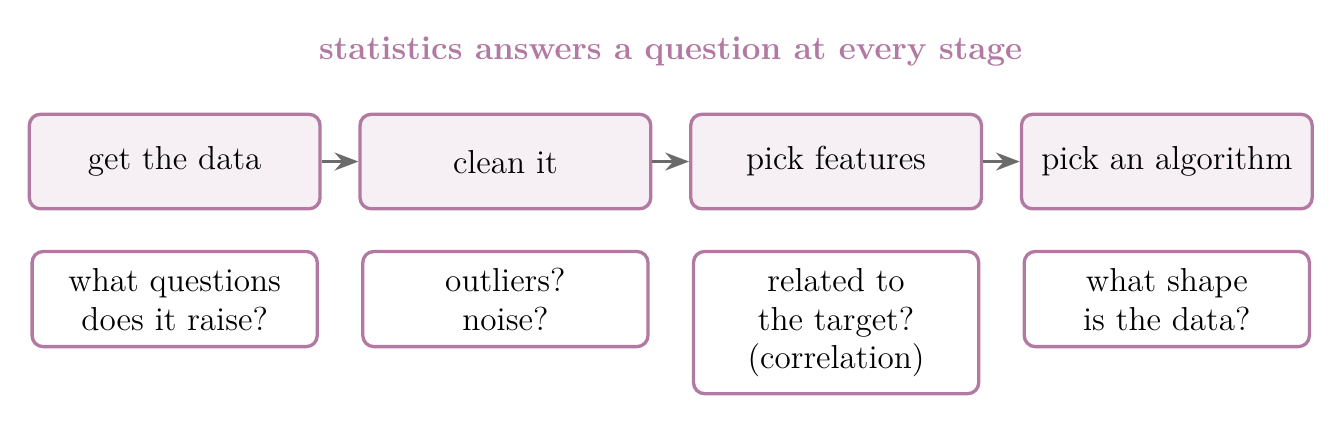
\begin{tikzpicture}[every node/.append style={font=\sffamily\large}, st/.style={box=cpurple, text width=3.2cm, minimum height=1.2cm}, q/.style={draw=cpurple, fill=white, rounded corners=4pt, text width=3.2cm, align=center, inner sep=6pt}]
  \node[st] (a) at (0,0) {get the data};
  \node[st] (b) at (4.2,0) {clean it};
  \node[st] (c) at (8.4,0) {pick features};
  \node[st] (d) at (12.6,0) {pick an algorithm};
  \foreach \u/\v in {a/b,b/c,c/d} \draw[arrow] (\u) -- (\v);
  \node[q, below=0.5cm of a] {what questions does it raise?};
  \node[q, below=0.5cm of b] {outliers?\\ noise?};
  \node[q, below=0.5cm of c] {related to the target? (correlation)};
  \node[q, below=0.5cm of d] {what shape is the data?};
  \node[font=\sffamily\large\bfseries, text=cpurple] at (6.3,1.4) {statistics answers a question at every stage};
\end{tikzpicture}
\end{document}
